\begin{frame}{Primera aproximación}
  \metroset{block=fill}
  \begin{block}{Eliminación de variables}
    \begin{itemize}
    \item scheme\_name: 1/2 de valores perdidos
    \item Variables categóricas con más de 100 características
    \item recorded\_by: una única categoría
    \item region\_code: Correlada con district\_code
    \item construction\_year: Correlada con gps\_height y valores perdidos
      (valores 0 en esta columna no tienen sentido)
    \end{itemize}
  \end{block}
  \begin{block}{Imputación de valores perdidos}
    \begin{itemize}
    \item Variables numéricas: valor medio
    \item Variables categóricas: valor modal
    \end{itemize}
  \end{block}
  \begin{block}{Resultado}
    0.7677
  \end{block}
\end{frame}

\begin{frame}{Mejoras a dicha aproximación}
  \metroset{block=fill}
  \begin{block}{Eliminación de filas con missing values}
    \begin{itemize}
    \item Quedan 49841 filas en el conjunto
    \item Precisión: 0.7328 $\rightarrow$ se descarta la vía
    \end{itemize}
  \end{block}
  \begin{block}{Imputación en train por clase}
    \begin{itemize}
    \item En lugar de la media y la moda globales, se imputa por media
      y mediana de la clase
    \item En test, seguimos imputando igual
    \item Precisión: 0.7677 $\rightarrow$ no mejora el resultado, se
      descarta
    \end{itemize}
  \end{block}
  \begin{block}{Creación de una nueva categoría para los valores perdidos}
    \begin{itemize}
    \item En las variables categóricas se añade una categoría nueva,
      que representa el valor perdido.
    \item Precisión: 0.7385 $\rightarrow$ se descarta la vía
    \end{itemize}
  \end{block}
\end{frame}

\begin{frame}{Segundo estudio - importancia de las variables}
  \metroset{block=fill}
  \begin{block}{Medición de la importancia de las variables}
    Para las variables numéricas con valores perdidos en
    entrenamiento, se computa el valor de dichas variables con la
    media de los valores de la clase, dejando el resto de variables
    imputadas de forma poco inteligente.\\

    Tras esto, se clasifica el conjunto de entrenamiento con
    validación cruzada.
  \end{block}
  \begin{block}{Intuición}
    Las variables que produzcan una mejora importante en el resultado
    contendrán información relevante para la solución del problema.
  \end{block}
\end{frame}

\begin{frame}{Segundo estudio - importancia de las variables}
  \metroset{block=fill}
  \begin{block}{Resultados}
    Mejora escasa o nula en todas las variables.\\

    Imputación correcta de \texttt{construction\_year} $\rightarrow$
    Mejora en la CV de 0.78 a 0.84.\\

    La variable \texttt{construction\_year} parece muy relevante a
    la hora de establecer la clasificación.
  \end{block}
\end{frame}

\begin{frame}{Segundo estudio - importancia de las variables}
  \metroset{block=fill}
  \begin{block}{Cómputo de \texttt{construction\_year}}
    Utilizamos el mejor modelo que tenemos hasta el momento.\\

    En función de la clase que se le ha predicho a cada elemento del
    test, se imputa el valor en función de la media de dicha clase
    en el conjunto de entrenamiento.
  \end{block}
  \begin{block}{Resultado}
    0.7875
  \end{block}
\end{frame}

\begin{frame}{Mejoras sobre este modelo (I)}
  \metroset{block=fill}
  \begin{block}{Edad de la fuente}
    Tenemos información de cuándo se hace la medida de la instancia
    (variable \texttt{date\_recorded}).\\

    No hay información perdida para dicha variable.\\

    Calculamos la edad de la fuente como la diferencia entre el año de
    la medida y la fecha de construcción.\\

    Se computa también el mes en el que se registra la fuente.\\

    Precisión: 0.7925
  \end{block}
  \begin{block}{Eliminación de las variables de registro y antigüedad}
    Eliminamos las medidas previas, manteniendo sólo la edad.\\

    Intentamos eliminar dependencia entre las variables.\\

    Precisión: 0.7822 $\rightarrow$ descartamos esta vía, conservamos
    las tres variables.
  \end{block}
\end{frame}

\begin{frame}{Mejoras sobre este modelo (II)}
  \metroset{block=fill}
  \begin{block}{Eliminación de la variable \texttt{num\_private}}
    Esta variable, a pesar de ser numérica, tiene pocos valores
    distintos, y la mayoría de valores son 0.\\

    No tenemos información sobre qué representa dicha variable, no podemos
    imputar nada sobre ella, por lo que decidimos prescindir de ella.\\

    Precisión: 0.7945 (mejor modelo)
  \end{block}
    \begin{block}{Eliminación del ruido de clase}
    Hay filas repetidas (los valores de todas las columnas que nos
    hemos quedado son iguales), con clases distintas.\\

    Nos quedamos con un solo ejemplo, cuya clase sea la que más se
    repite entre las filas repetidas.\\

    Precisión: 0.7916 $\rightarrow$ descartamos el modelo
  \end{block}
\end{frame}

\begin{frame}{Otras propuestas}
  \metroset{block=fill}
  \begin{block}{PCA}
    Las variables categóricas se transforman a variables binarias y se
    extraen las $k = 28$ primeras características (tantas como
    variables categóricas teníamos de partida). \\

    Precisión: 0.7822
  \end{block}

  \begin{block}{PCA + SMOTE}
    Sobre los datos anteriores, utilizamos SMOTE para intentar balancear
    las clases:
    \begin{itemize}
    \item La variable \texttt{functional needs repair} se iguala a la
      clase \texttt{functional}
    \item A la variable \texttt{non functional} se le duplican el
      número de ejemplos.
    \end{itemize}
    Precisión: 0.7651\\

    Se genera demasiado ruido, y empeora la clasificación.
  \end{block}
\end{frame}

\begin{frame}{Evolución de la puntuación}
  \begin{figure}
    \centering
    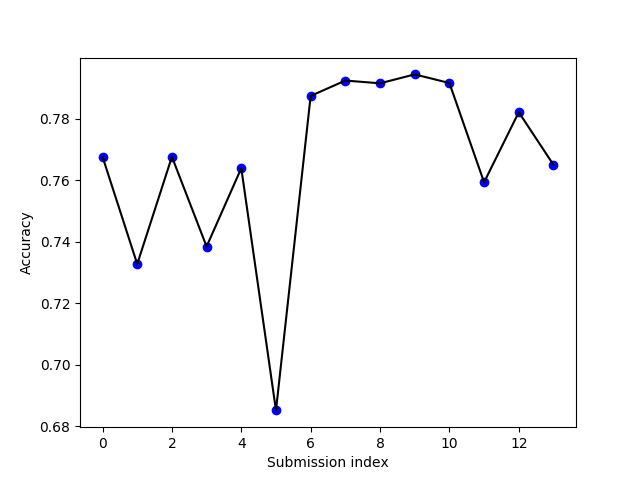
\includegraphics[height=.6\textheight]{figures/evolutiontrees}
    \caption{Evolución de la puntuación a lo largo de las subidas}
  \end{figure}
  Mejor puntuación final: 0.7945 - Posición actual: 1702
\end{frame}
